\documentclass[12pt]{sigplanconf}

% The following \documentclass options may be useful:

% preprint      Remove this option only once the paper is in final form.
% 10pt          To set in 10-point type instead of 9-point.
% 11pt          To set in 11-point type instead of 9-point.
% authoryear    To obtain author/year citation style instead of numeric.

\usepackage{amsmath}
\usepackage{shortcut}
\usepackage{subcaption}
\usepackage{graphicx}
\usepackage{hyperref}

\newtheorem{definition}{Definition}[section]

\begin{document}

\special{papersize=8.5in,11in}
\setlength{\pdfpageheight}{\paperheight}
\setlength{\pdfpagewidth}{\paperwidth}

\titlebanner{banner above paper title}        % These are ignored unless
\preprintfooter{short description of paper}   % 'preprint' option specified.

\title{Improving Directed Fuzzing by Projecting String Domain Input to Finite State Machine}

\authorinfo{Jaeho Kim}
{KAIST \\
    Daejeon, South Korea
}
{oojahooo@kaist.ac.kr}
\authorinfo{Tae Eun Kim}
{KAIST \\
    Daejeon, South Korea
}
{goodtaeeun@kaist.ac.kr}
\authorinfo{Seunghyeon Jeong}
{KAIST \\
    Daejeon, South Korea
}
{antony@kaist.ac.kr}
\authorinfo{Kihwan Kim}
{KAIST \\
    Daejeon, South Korea
}
{kimkihwan@kaist.ac.kr}

\maketitle

\begin{abstract}
    Fuzzing is a good technique for finding bug in target program. There is a
    traditional fuzzing technique that uses only code coverage, called greybox
    fuzzing. But in string domain, it struggle with the absence of code coverage.
    So we present a effective transformation of target code, using the concept of
    finite state machine, and combining to directed fuzzing. Our implementation
    can reproduce bug of target location more efficiently than traditional fuzzer.
    And our implementation is in \url{https://github.com/goodtaeeun/smAFL}.
\end{abstract}

\section{Introduction}
Fuzzing is a technique that is widely applied in the real world with its simple intuition and excellent applicability.
For example, Google provides a large platform named OSS-Fuzz for open source software. Developers can upload their open
source project to this platform and get reports about bugs that founded by executing the fuzzer. Actually, OSS-Fuzz has
helped identify and fix over 8,900 vulnerabilities and 28,000 bugs across 850 projects~\footnote{https://github.com/google/oss-fuzz\#trophies}.

Greybox fuzzing is a generally used fuzzing technique that explores the program guided by code coverage. It mutates the
seed inputs in a way that increases code coverage. The term `Greybox' means that the fuzzer does not use whole information
of program's code, but it uses only code coverage information.

\begin{figure}[h]
    \cFormat
    \lstinputlisting[]{figure/ex1.c}
    \hrule width \hsize height .33pt
    \caption{Condition Example of a Simple Program that Takes String Input}
    \label{fig:string-example}
  \end{figure}

Because of the aforementioned characteristic of greybox fuzzer, it struggle with the absence of code coverage. Especially,
it is challenging for greybox fuzzer if there are conditions with no intermediate code coverage. Figure~\ref{fig:string-example}
shows the example of the condition with no intermediate code coverage. At the line 6, the input argument should be exactly
``HELLO'' in order to execute true branch and crash statement at line 8. So executing with input string ``HELL'' and
``HEAVEN'' respectively have same code coverage. It is fatal problem for mutator in greybox fuzzing. ``HELL'' is more
similar (i.e. less edit distance) with ``HELLO'' than ``HEAVEN'', so it can make ``HELLO'' by adding only one character,
but the fuzzer evaluates those two inputs are same effectiveness. Therefore the fuzzer makes more insignificant inputs,
and it takes too much time.

To overcome this problem, we present a new task for encoding the value coverage in string domain, using finite state machine,
and combine it with directed fuzzing technique. Directed fuzzing is a new technique of fuzzing that aims a specific location
of the program. So it is more efficient than greybox fuzzing when we want to find an input that causes program to crash
at specific location.

\section{Overview}
\subsection{Finite State Machine}
Finite state machine is a useful structured representation that represents a program's behavior. In general, a program is
a transition system. Every program has states and transition functions. So we can express a program defining states and
transition function. Actually, Depending on how the state and transition function are defined, an infinite number of states
may be required to express a program. But in a specific domain, we can represent it using finite number of states. So we
utilize the finie state machine for only representing conditional expression containing string library functions.

We define finite state machine like below for using our domain.

\begin{definition}
    $(Q, \Sigma, \delta, q_0, F)$ is a finite state machine where $Q$ is finite set of states, $\Sigma$ is a set of input
    symbol, especially ascii characters in our domain, $\delta : (Q \times \Sigma) \rightarrow Q$ is a partial function
    that takes current state and current input symbol, $q_0$ is initial state (i.e. state that input symbol is empty string),
    and $F$ is a set of accepted (final) states.
\end{definition}

\subsection{Examples and Methods}

\begin{figure}[h]
    \begin{subfigure}[t]{0.45\textwidth}
        \cFormat
        \lstinputlisting[]{figure/strcmp.c}
        \hrule width \hsize height .33pt
        \caption{Scenario that uses strcmp function}
        \label{fig:strcmp}
    \end{subfigure}
    \begin{subfigure}[t]{0.45\textwidth}
        \cFormat
        \lstinputlisting[]{figure/strstr.c}
        \hrule width \hsize height .33pt
        \caption{Scenario that uses strstr function}
        \label{fig:strstr}
    \end{subfigure}
    \begin{subfigure}[t]{0.45\textwidth}
        \cFormat
        \lstinputlisting[]{figure/atoi.c}
        \hrule width \hsize height .33pt
        \caption{Scenario that uses atoi function}
        \label{fig:atoi}
    \end{subfigure}
    \caption{Three scenarios that usually occurs in many programs}
    \label{fig:scenarios}
\end{figure}

We choose three scenarios that usually occurs in many programs that take string inputs, 1) using \verb|strcmp| function
in conditional expression, 2) using \verb|strstr| function in conditional expression, 3) using \verb|atoi| function in
conditional expression. Figure~\ref{fig:scenarios} is the simple code examples that contains our scenarios.

Each scenario makes greybox fuzzer struggle with the absence of code coverage. In Figure~\ref{fig:strcmp}, we have to find
exactly ``123456'' as an crashing input. In Figure~\ref{fig:strstr}, we should find the string that contains ``1234'' as
an crashing input. In Figure~\ref{fig:atoi}, we have to find the string that represents the integer 123456.

To make new coverage method for these scenarios, we use the finite state machine. Finite state machine can express the
sequence of transition from starting input symbol to final input symbol, and check whether the input string is accepted.

\begin{figure}[h]
    \begin{subfigure}[t]{0.45\textwidth}
        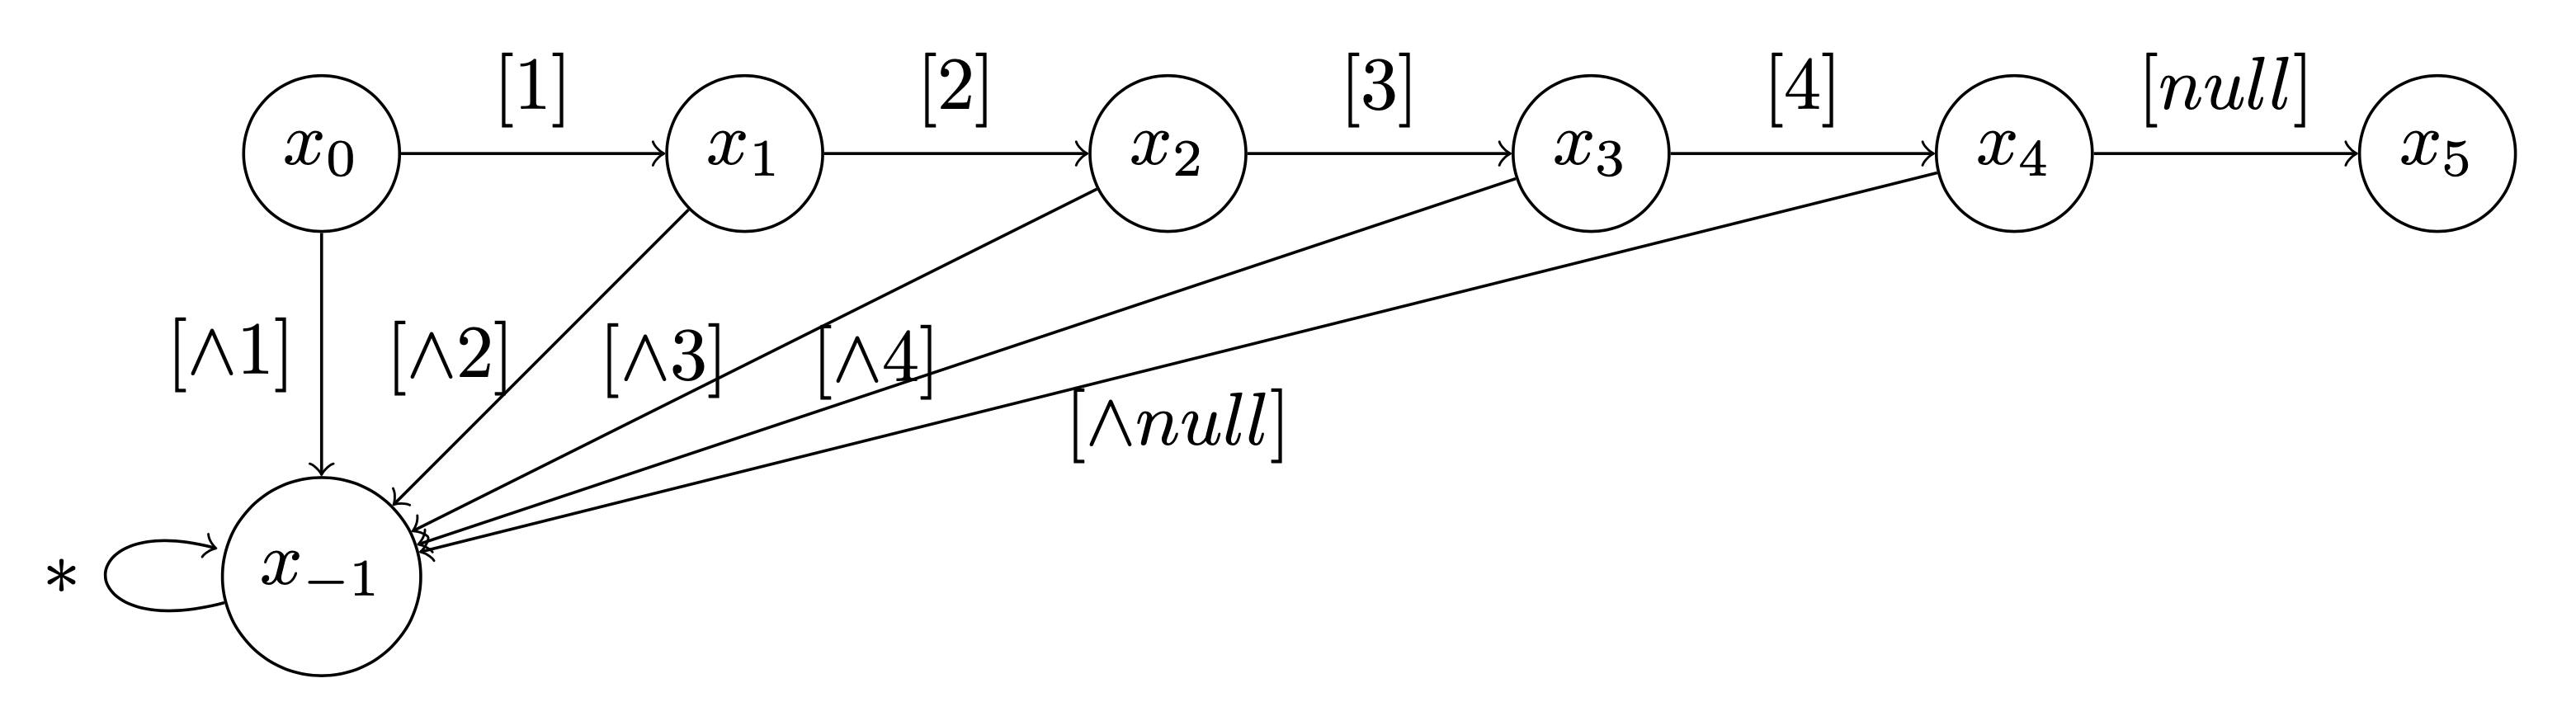
\includegraphics[width=\textwidth]{figure/strcmp.png}
        \caption{Contructed FSM for strcmp}
        \label{fig:fsm-strcmp}
    \end{subfigure}
    \begin{subfigure}[t]{0.45\textwidth}
        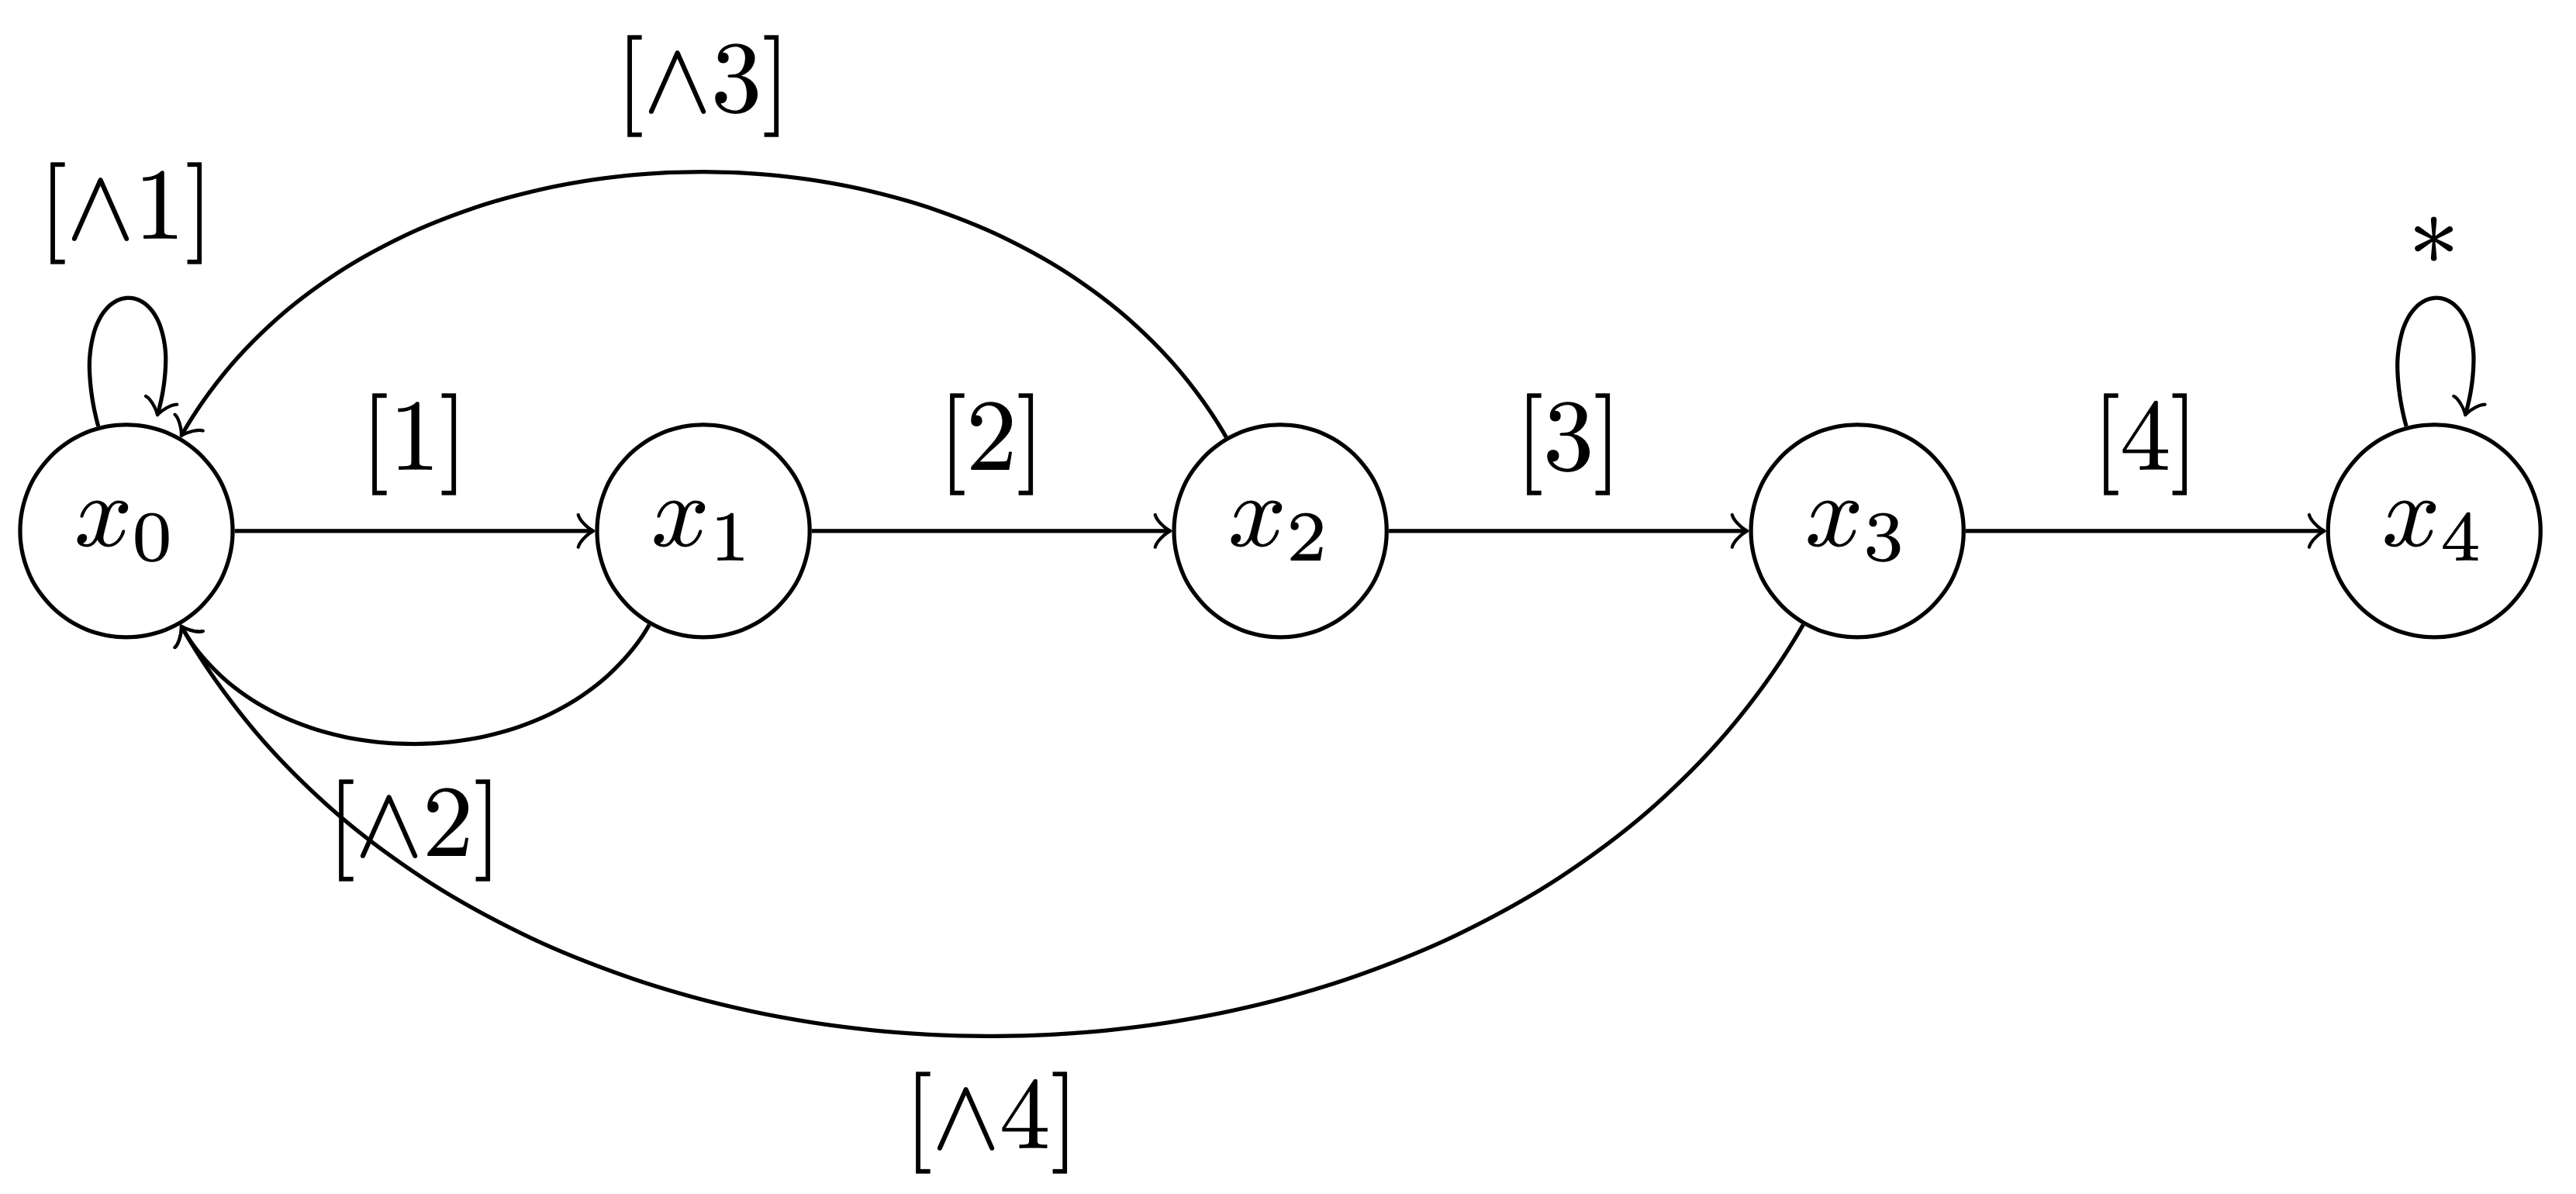
\includegraphics[width=\textwidth]{figure/strstr.png}
        \caption{Contructed FSM for strstr}
        \label{fig:fsm-strstr}
    \end{subfigure}
    \begin{subfigure}[t]{0.45\textwidth}
        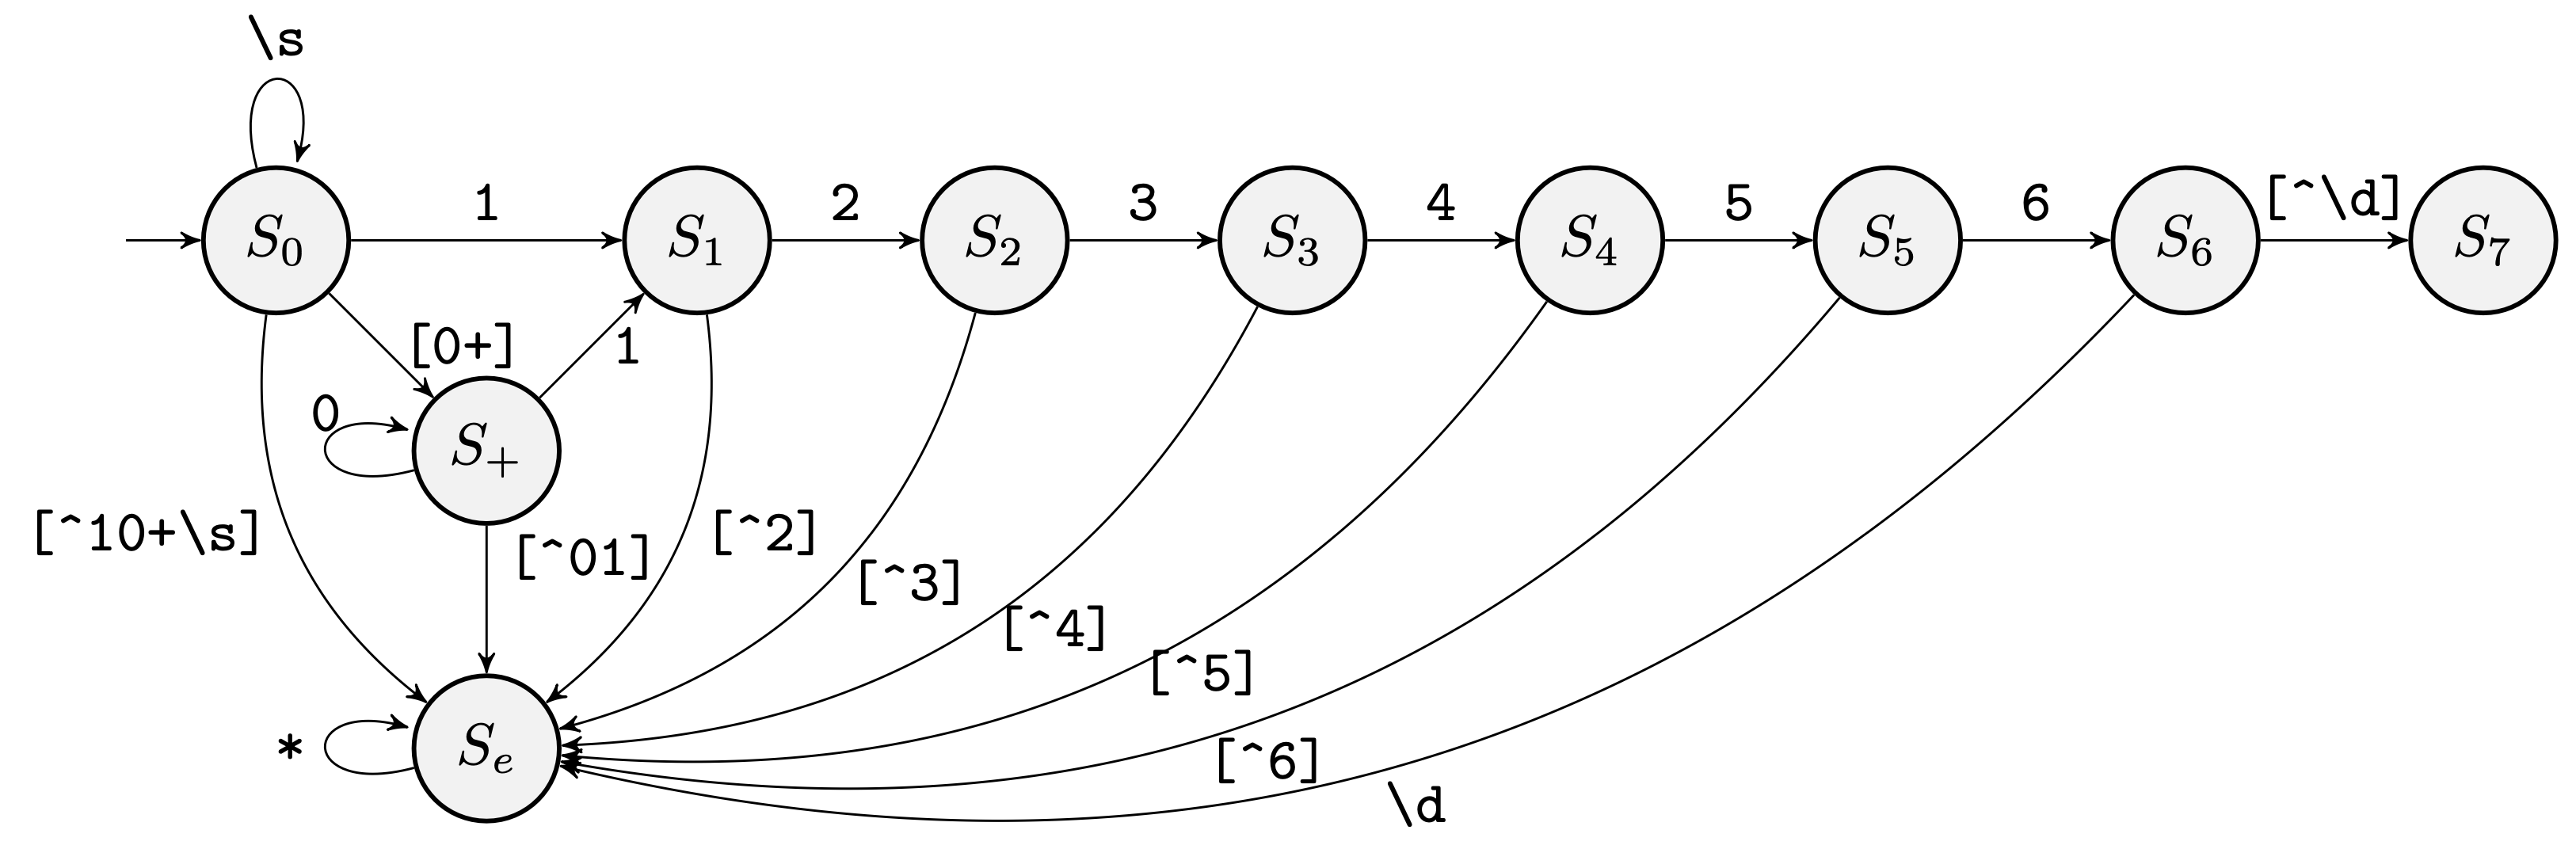
\includegraphics[width=\textwidth]{figure/atoi.png}
        \caption{Contructed FSM for atoi}
        \label{fig:fsm-atoi}
    \end{subfigure}
    \caption{Constructed finite state machines for each scenario}
    \label{fig:fsm} 
\end{figure}

So we construct the finite state machines for each scenario, and add it as new conditional statement these to original code.
Figure~\ref{fig:fsm} shows the FSMs constructed for each scenario. And we implement these FSMs in real program as adding
new code.

You can see the detailed implementation in our repo~\footnote{https://github.com/goodtaeeun/smAFL}.

\section{Evaluation}
\label{eval}
We have an experiment for comparing the efficiency of our technique with traditional fuzzers. So our baselines are traditional
greybox fuzzer, AFL~\cite{aflfuzz}, and traditional directed fuzzer, AFLGO~\cite{bohme:ccs:2017}.

\begin{table}
    \small
     \caption{Crash reproduction results of smAFL and the baseline tools.
             %
             Each reported number is a median over 40 repeated experiments.
             %
             N.A. indicates that the tool could not produce a median TTE,
             which means that it was not able to reproduce the bug for more than half of the repeated
             experiments. The parentheses denote how many times the fuzzer was able to
             reproduce the bug. Unlike TTE, this number is better when bigger.
             %
             For each target (i.e., each row), the best result is marked with
             bold font and an asterisk.
             %
             \# Best perf. denotes the number of targets for which the tool has the best performance among all the other tools.}
         \begin{tabular}{@{}l@{\ \ \ \ \ \ \ \ \ }l@{\ \ \ \ \ \ \ }l@{\ \ \ \ \ \ \ }l@{\ \ \ \ \ \ \ \ \ \ \ }c@{\ \ \ \ \ \ \ \ }c@{}}\toprule
            \textbf{Scenario}	&	\multicolumn{1}{c}{\textbf{CVE}}	&	\multicolumn{1}{c}{		AFL		}	&	\multicolumn{1}{r}{		AFLGo		}	&	\multicolumn{1}{c}{		smAFL		}	\\\midrule
            \multirow[c]{3}{*}{\texttt{strcmp}}	&	2016-4487	&	\multicolumn{1}{r}{	\text{	100	}	}	&	\multicolumn{1}{r}{	\text{	100	}	}	&	\multicolumn{1}{r}{	\text{	100	}	}	\\
                &	2016-4489	&	\multicolumn{1}{r}{	\text{	100	}	}	&	\multicolumn{1}{r}{	\text{	100	}	}	&	\multicolumn{1}{r}{	\text{	100	}	}	\\
                &	2016-4490	&	\multicolumn{1}{r}{	\text{	100	}	}	&	\multicolumn{1}{r}{	\text{	100	}	}	&	\multicolumn{1}{r}{	\text{	100	}	}	\\
                &	2016-4492	&	\multicolumn{1}{r}{	\text{	100	}	}	&	\multicolumn{1}{r}{	\text{	100	}	}	&	\multicolumn{1}{r}{	\text{	100	}	}	\\\midrule
            \multirow[c]{3}{*}{\texttt{strstr}}	&	2016-4487	&	\multicolumn{1}{r}{	\text{	100	}	}	&	\multicolumn{1}{r}{	\text{	100	}	}	&	\multicolumn{1}{r}{	\text{	100	}	}	\\
                &	2016-4489	&	\multicolumn{1}{r}{	\text{	100	}	}	&	\multicolumn{1}{r}{	\text{	100	}	}	&	\multicolumn{1}{r}{	\text{	100	}	}	\\
                &	2016-4490	&	\multicolumn{1}{r}{	\text{	100	}	}	&	\multicolumn{1}{r}{	\text{	100	}	}	&	\multicolumn{1}{r}{	\text{	100	}	}	\\
                &	2016-4492	&	\multicolumn{1}{r}{	\text{	100	}	}	&	\multicolumn{1}{r}{	\text{	100	}	}	&	\multicolumn{1}{r}{	\text{	100	}	}	\\\midrule
            \multirow[c]{3}{*}{\texttt{atoi}}	&	2016-4487	&	\multicolumn{1}{r}{	\text{	100	}	}	&	\multicolumn{1}{r}{	\text{	100	}	}	&	\multicolumn{1}{r}{	\text{	100	}	}	\\
                &	2016-4489	&	\multicolumn{1}{r}{	\text{	100	}	}	&	\multicolumn{1}{r}{	\text{	100	}	}	&	\multicolumn{1}{r}{	\text{	100	}	}	\\
                &	2016-4490	&	\multicolumn{1}{r}{	\text{	100	}	}	&	\multicolumn{1}{r}{	\text{	100	}	}	&	\multicolumn{1}{r}{	\text{	100	}	}	\\
                &	2016-4492	&	\multicolumn{1}{r}{	\text{	100	}	}	&	\multicolumn{1}{r}{	\text{	100	}	}	&	\multicolumn{1}{r}{	\text{	100	}	}	\\\midrule
            \multicolumn{2}{c}{\textbf{\# Best perf.}}			&	\multicolumn{1}{r}{	\text{	100	}	}	&	\multicolumn{1}{r}{	\text{	100	}	}	&	\multicolumn{1}{r}{	\text{	100	}	}	\\\bottomrule

     \end{tabular}
     \label{tbl:main-table}
 \end{table}


\subsection{Experimental Setup}

\subsubsection{Benchmarks}
We use the following benchmarks for our experiment: CVE-2016-4487, CVE-2016-4489, CVE-2016-4490, CVE-2016-4492.
These benchmarks are originally from the paper of AFLGO~\cite{bohme:ccs:2017}.
We chose these benchmarks as they are realistic and are used frequently in the field of directed fuzzing.
However, the benchmarks required changes to fit our target domain.
Thus, we modified the benchmarks by applying some patches that insert a guarding condition that uses user input strings.
The patches can be found in our repository under the directory
\texttt{docker-setup/benchmark-project}
\texttt{/binutils-2.26/patches}.

\subsection{Baselines}
In order to evaluate the effectiveness of our technique, we compare our technique with two baselines: AFL and AFLGO.
AFL is an undirected greybox fuzzer that is widely used in the field of fuzzing. We use AFL to compare the effectiveness
of the AFLGo and the further enhancement made by our tool.

\subsection{Evaluation Criteria}
In order to evaluate the directed fuzzers, we compare the time taken to reproduce a bug lying in the target location.
Whenever a fuzzer finds a bug, we record the time taken to reproduce the bug.
After the fuzzing session, we replay the found crashing inputs against the program that is built with ASAN options.
Then, by comparing the ASAN error log, we can determine whether the desired bug is reproduced or not.
Refer to the script \texttt{scripts/triage.py} for the detailed criteria for each target bug.

\subsection{Experimental Specification}
We run each fuzzer for 10000 seconds on each target.
We also repeat the experiment for 40 times to mitigate the effect of randomness in fuzzing.
Then, we use the median value of the time take to reproduce the target bug among the 40 iterations.

\subsection{Result}
Table~\ref{tbl:main-table} shows the result of our experiment. The baselines, AFL, AFLGo, cannot reproduce the bugs at most.
The best performance of AFL is in scenario \verb|atoi|, case 2016-4492, but even in this case, AFL reproduce only three
times during 40 repeated experiments. In most cases, AFL and AFLGo never reproduced one.

In contrast, our tool, smAFL reproduced the bug for more than half of the repeated experiments (i.e. more than 20 times)
in every case. And the efficiency of our tool is also worthwhile. The worst case, scenario \verb|strcmp| CVE id 2016-4492,
takes less than 40 minutes. It is pretty early compared to the timeout of each experiment, 167 minutes. If a developer use
our tool, then he/she can find the bug and crashing input in 40 minutes.

\section{Conclusion}
As we can see in section~\ref{eval}, our scenarios effectively block the traditional greybox fuzzer. The conditions using
string library functions make fuzzer hard to find accepted string input. Because the code coverage information that used
for greybox fuzzer does not says how the seed inputs are closed from target string.

Unlike this, our implementation encodes the distance between a seed input and target string as a code coverage information.
Therefore the directed fuzzer can find the bug more efficiently than traditional fuzzer.

\section{Future Works}
Our experiments showed that the code coverage modification technique using FSM is sufficiently effective in the string
domain. But we implemented only three scenarios, so we think it needs to become automated tool for all string functions.

\bibliographystyle{ACM-Reference-Format}
\bibliography{references}

\end{document}